\documentclass[tikz,border=10pt]{standalone}
\usepackage{tikz}
\usepackage{xcolor}
\usepackage{amsmath}
\usetikzlibrary{shapes,arrows,positioning,calc}

\begin{document}

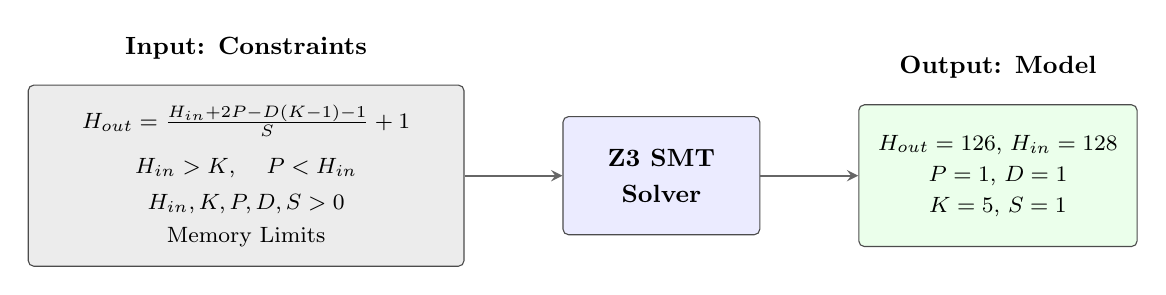
\begin{tikzpicture}[
    scale=1.0,
    constraint/.style={rectangle, draw=black!70, fill=gray!15, minimum width=5.5cm, minimum height=1.5cm, text centered, font=\footnotesize, rounded corners=2pt},
    solver/.style={rectangle, draw=black!70, fill=blue!8, minimum width=2.5cm, minimum height=1.5cm, align=center, font=\small\bfseries, rounded corners=2pt},
    solution/.style={rectangle, draw=black!70, fill=green!8, minimum width=3.5cm, minimum height=1.2cm, text centered, font=\footnotesize, rounded corners=2pt},
    arrow/.style={->, >=stealth, thick, black!60},
    formula/.style={font=\footnotesize}
]

% Input: Constraints - merged into one block
\node[constraint, minimum height=2.3cm] (constraints) {
    \begin{minipage}{5.3cm}
    \centering
    $H_{out} = \frac{H_{in} + 2P - D(K-1) - 1}{S} + 1$\\[0.8em]
    $H_{in} > K$, \quad $P < H_{in}$\\[0.4em]
    $H_{in}, K, P, D, S > 0$\\[0.3em]
    Memory Limits
    \end{minipage}
};

% Output: Solution
\node[solution, right=5.0cm of constraints, minimum height=1.8cm] (solution) {
    \begin{minipage}{3.3cm}
    \centering
    $H_{out} = 126$, $H_{in} = 128$\\[0.2em]
    $P = 1$, $D = 1$\\[0.2em]
    $K = 5$, $S = 1$
    \end{minipage}
};

% Z3 Solver - positioned at the middle vertically between constraints and solution
\node[solver, at=($(constraints.east)!0.5!(solution.west)$)] (z3) {Z3 SMT\\[0.2em]Solver};

% Arrows
\draw[arrow] (constraints.east) -- (z3.west);
\draw[arrow] (z3.east) -- (solution.west);

% Labels
\node[above=0.2cm of constraints, font=\small\bfseries] {Input: Constraints};
\node[above=0.2cm of solution, font=\small\bfseries] {Output: Model};

\end{tikzpicture}

\end{document}

